\documentclass[11pt,a4paper]{article}
\usepackage[utf8]{inputenc}
\usepackage[T1]{fontenc}
\usepackage[margin=2.2cm,top=2.4cm,bottom=2.4cm]{geometry}
\usepackage{graphicx}
\usepackage{booktabs}
\usepackage{listings}
\usepackage{xcolor}
\usepackage{tikz}
\usetikzlibrary{arrows.meta,positioning}
\usepackage{enumitem}
\usepackage{caption}
\usepackage{array}
\usepackage{amsmath}
\usepackage[hidelinks]{hyperref}

\setlist{itemsep=0.2em,topsep=0.3em}
\captionsetup{font=small,skip=6pt}
\lstset{basicstyle=\footnotesize\ttfamily,keywordstyle=\color{blue!70!black},
  commentstyle=\color{green!50!black}\itshape,stringstyle=\color{red!60!black},
  frame=single,rulecolor=\color{black!30},breaklines=true,showstringspaces=false,
  numbers=left,numberstyle=\tiny\color{black!50},xleftmargin=1.2em}

\title{A Case Study Report on\\Agricultural Water Usage Analyzer}
\author{Batch No.~16}
\date{December 2026}

\begin{document}

% ---------------- Title page ----------------
\begin{titlepage}
\centering

\includegraphics[width=3.4cm]{figures/vce_logo.jpg}\\[0.6cm]
{\large\bfseries A Case Study Report on}\\[0.4cm]
{\LARGE\bfseries Agricultural Water Usage Analyzer}\\[0.8cm]
{\large A9502 -- Programming for Problem Solving Laboratory}\\[1.0cm]
{\bfseries Submitted by}\\[0.3cm]
Batch No.~16\\[0.4cm]
\begin{tabular}{ll}
D.~Taraka Ramarao & (25881A05EH)\\
K.~Umesh Chandra Prasad & (25881A05EJ)\\
B.~Ushasree & (25881A05EK)\\
\end{tabular}\\[1.0cm]
{\bfseries Course Facilitator}\\[0.2cm]
K Raghavendra\\
Department of Computer Science and Engineering\\[0.8cm]
{\large\bfseries Department of Computer Science and Engineering}\\[0.3cm]
{\large\bfseries Vardhaman College of Engineering, Hyderabad}\\[0.3cm]
{\large\bfseries December 2026}
\vfill
{\small Head of Department: Y Vijayalatha, Department of Computer Science and Engineering}
\end{titlepage}

% ---------------- Abstract ----------------
\begin{abstract}
\noindent Agriculture is the largest user of freshwater, and wasteful irrigation
threatens both farm incomes and groundwater security. This case study develops an
\emph{Agricultural Water Usage Analyzer} in Python that compares irrigation water
consumption across eight crops, five farming regions, four irrigation methods and
twelve months. A dataset of 612 irrigation records was cleaned and validated
(duplicates, missing values, negative values, invalid months and statistical outliers
removed), leaving 550 valid records covering 1,749.23~ha and 1,292,341~m$^3$ of water.
Totals, percentage shares and water-intensity rates (m$^3$ per hectare) were computed
with lists, dictionaries, functions and file handling, and the results were visualised
with Matplotlib. Sugarcane (1,581.8~m$^3$/ha) and rice (1,158.0~m$^3$/ha) are the most
water-intensive crops; together they use 41.6\% of all water on only 22.5\% of the area.
Warangal (850.4~m$^3$/ha) and Karimnagar (828.2~m$^3$/ha) are the highest-intensity
regions, while Mahabubnagar (595.3~m$^3$/ha) is the lowest. October, November and June
account for 39.0\% of annual use. Flood irrigation uses 2.8 times as much water per
hectare as drip irrigation. A conservative planning estimate shows that reducing
flood-irrigation water by 30\% would save about 161,227~m$^3$ (12.5\% of total use).
The dataset is simulated by the program itself (fixed random seed 16); the same
program runs unchanged on a real CSV file with the same columns.

\medskip\noindent\textbf{Keywords:} water usage analysis; irrigation; crop water
intensity; data cleaning; Python; Matplotlib; regional comparison.
\end{abstract}

\tableofcontents
\newpage

% ---------------- 1 ----------------
\section{Introduction}
Irrigation accounts for most agricultural water use, yet farmers, extension officers
and water-user associations often lack a simple way to see \emph{where} water is going:
which crops, which regions, which months and which irrigation methods consume the most.
Decisions made on total water alone are misleading, because a large region or a
widely grown crop will always appear to use more water. Water use must therefore be
normalised by irrigated area, giving water intensity in cubic metres per hectare
(m$^3$/ha), and compared across crops, regions, methods and months.

This case study, carried out for A9502 (Programming for Problem Solving Laboratory),
builds a small, readable Python program that does exactly that: it loads irrigation
records from a CSV file, cleans and validates them, computes totals, shares and
intensities, and produces summary tables and charts that support practical
recommendations. It is a mid-level Python project: a single script of about 340 lines
using the standard library plus Matplotlib, organised into functions for each stage of
the pipeline. It uses no database, web framework, machine-learning model or external
API, and this report does not claim otherwise.

\section{Background, Problem Statement and Objectives}
\subsection{Background}
The five regions studied --- Nizamabad, Warangal, Karimnagar, Medak and
Mahabubnagar --- grow a mix of food, fibre and horticultural crops under flood,
furrow, sprinkler and drip irrigation. Traditional record-keeping is paper-based and
error-prone: in this study's raw data, about one record in ten was unusable. Without
cleaning and standardisation, any comparison of crops or regions inherits those errors.
The stakeholders are farmers (who pay for pumping and canal water), the agriculture
office and irrigation department (which plan releases and subsidies), and water-user
associations (which schedule turns in peak months).

\subsection{Problem statement}
How can irrigation records be turned, with a transparent and reproducible Python
program, into reliable answers to three questions: (i)~which crops are the most
water-intensive, (ii)~which regions and months use water most heavily, and
(iii)~how much water could plausibly be saved by changing irrigation practice?

\subsection{Objectives}
\begin{enumerate}
  \item Collect irrigation records and define the key variables: region, crop, month,
        area, irrigation method and water used.
  \item Clean and validate the records in Python so that only reliable data is analysed.
  \item Calculate totals, percentage shares and water intensity (m$^3$/ha) for crops,
        regions, methods and months.
  \item Identify water-intensive crops, compare regions and find high-consumption periods.
  \item Interpret the findings and recommend practical, water-efficient practices.
\end{enumerate}

\section{Scope and Limitations}
Included: eight crops (rice, sugarcane, cotton, maize, wheat, groundnut, tomato,
chilli), five regions, four irrigation methods and a twelve-month period, covering data
loading, cleaning, analysis, visualisation and recommendations. Excluded: rainfall,
soil type, groundwater depth, electricity use, crop yield and economic returns, so
water productivity (yield per m$^3$) cannot be calculated.

Two limitations shape every conclusion in this report. First, no public farm-level
irrigation dataset was supplied with the case study, so the analysis uses a simulated
dataset produced by the program itself (fixed seed 16) from realistic crop water needs,
regional factors and seasonal patterns. The numbers therefore illustrate the method;
they are not measurements of real farms. Second, irrigation method is closely tied to
crop in the data (rice and sugarcane are flood-irrigated), so crop and method effects
cannot be fully separated; field trials would be needed to measure the pure method
effect. Results also describe a single year and cannot show long-term trends.

\section{Methodology and System Architecture}
The study follows a document-and-data approach implemented as one Python program
(\texttt{water\_\allowbreak usage\_\allowbreak analyzer.py}).
Figure~\ref{fig:arch} shows the pipeline; each
stage is a separate function, so a stage can be tested and changed independently.
Table~\ref{tab:modules} lists the program's modules and functions.

\begin{figure}[h]
\centering
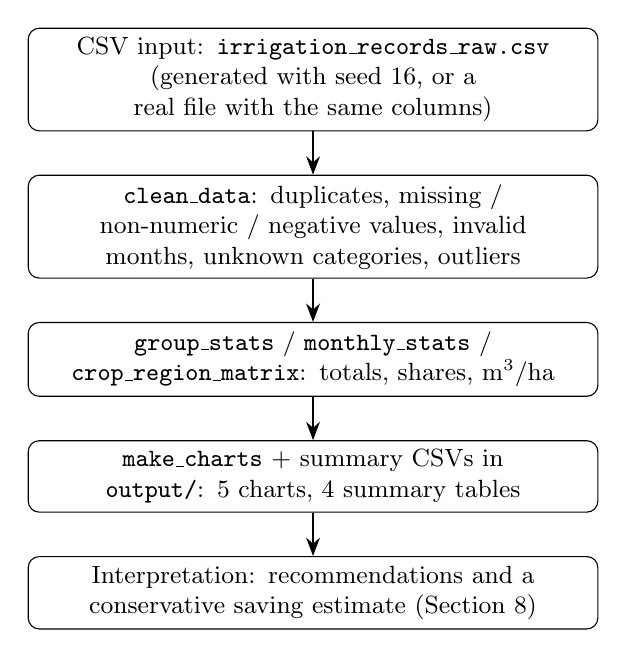
\begin{tikzpicture}[node distance=0.55cm, every node/.style={draw, rounded corners,
  text width=7.0cm, minimum height=0.75cm, align=center, font=\small},
  arrow/.style={-{Stealth}, thick}]
  \node (a) {CSV input: \texttt{irrigation\_records\_raw.csv} \\
    (generated with seed 16, or a real file with the same columns)};
  \node[below=of a] (b) {\texttt{clean\_data}: duplicates, missing / non-numeric /
    negative values, invalid months, unknown categories, outliers};
  \node[below=of b] (c) {\texttt{group\_stats} / \texttt{monthly\_stats} /
    \texttt{crop\_region\_matrix}: totals, shares, m$^3$/ha};
  \node[below=of c] (d) {\texttt{make\_charts} + summary CSVs in \texttt{output/}:
    5 charts, 4 summary tables};
  \node[below=of d] (e) {Interpretation: recommendations and a conservative
    saving estimate (Section~8)};
  \draw[arrow] (a) -- (b); \draw[arrow] (b) -- (c);
  \draw[arrow] (c) -- (d); \draw[arrow] (d) -- (e);
\end{tikzpicture}
\caption{System architecture: input, cleaning, analysis, output and interpretation.
  The cleaned CSV (\texttt{irrigation\_records\_clean.csv}) is written between the
  cleaning and analysis stages.}
\label{fig:arch}
\end{figure}

\begin{table}[h]
\centering\small
\caption{Program structure: one script, functions grouped by pipeline stage.}
\label{tab:modules}
\begin{tabular}{>{\raggedright\arraybackslash}p{2.0cm}
  >{\raggedright\arraybackslash}p{3.9cm}
  >{\raggedright\arraybackslash}p{9.0cm}}
\toprule
Stage & Function & Responsibility \\
\midrule
Data & \texttt{generate\_raw\_data} & Simulates 600 records (seed 16) and injects faults \\
     & \texttt{load\_csv}, \texttt{save\_csv} & \texttt{csv} module file handling \\
Cleaning & \texttt{clean\_data} & Validation, normalisation, outlier rule; returns a report \\
Analysis & \texttt{group\_stats} & Totals, shares and intensity per crop / region / method \\
     & \texttt{monthly\_stats} & Monthly totals and shares \\
     & \texttt{crop\_region\_matrix} & Intensity for every crop $\times$ region cell \\
     & \texttt{potential\_saving} & Returns the observed drip intensity \\
Output & \texttt{make\_charts}, \texttt{print\_table} & 5 Matplotlib charts; console tables \\
     & \texttt{main} & Runs the pipeline in order and prints recommendations \\
\bottomrule
\end{tabular}
\end{table}

The core Python concepts demonstrated are: lists of dictionaries for records;
dictionaries and \texttt{collections.defaultdict} for grouping; sets for duplicate
detection; \texttt{try/except} for numeric validation; \texttt{csv} file handling;
sorting with \texttt{lambda} keys; and Matplotlib for bar charts, a line chart and a
heatmap. Conversion used throughout: 1~mm of water over 1~ha equals 10~m$^3$.

\section{Python Implementation}
\subsection{Data generation}
\texttt{generate\_raw\_data} draws a crop, region and growing month from the
\texttt{CROPS} and \texttt{REGIONS} dictionaries, then computes water from typical need
(mm), a regional multiplier, a seasonal factor and 2--6 irrigation events. It then
deliberately injects faults --- missing values, negatives, absurd outliers, inconsistent
capitalisation and spacing, invalid months and duplicates --- so that the cleaning
stage has real work to do. Because the random seed is fixed (16), a fresh run always
produces the same 612 rows (600 base records plus 12 duplicates). If a raw CSV already
exists, \texttt{main} reuses it instead of regenerating it; deleting the CSV files is
therefore the way to reproduce the generation step.

\subsection{Cleaning and validation}
Listing~\ref{lst:clean} is the heart of the program. Text fields are standardised with
\texttt{strip().title()}, so `` Rice '' and ``RICE'' become ``Rice''. Rows are then
rejected, in order, for missing values, non-numeric values, non-positive area or water,
months outside 1--12, and crops or regions not in the reference dictionaries. Finally,
an outlier rule removes records whose intensity exceeds $Q3 + 3 \times IQR$ (the third
quartile plus three interquartile ranges), a deliberately strict threshold chosen so
that only extreme values --- the injected 90,000--250,000~m$^3$ rows and a few similar
cases --- are dropped. Every rejection is counted in a report dictionary, so the
cleaning step is auditable rather than silent.

\begin{lstlisting}[language=Python, caption={Cleaning and validation (extract from
  \texttt{clean\_data}; the full function is in the repository).},
  label={lst:clean}]
for r in records:
    key = tuple(r.values())
    if key in seen:                      # exact duplicate
        report["duplicates_removed"] += 1
        continue
    seen.add(key)
    r["crop"] = r["crop"].strip().title()  # normalise text
    if r["area_ha"] == "" or r["water_used_m3"] == "":
        report["missing_values_removed"] += 1
        continue
    try:
        r["area_ha"] = float(r["area_ha"])
        r["water_used_m3"] = float(r["water_used_m3"])
        r["month"] = int(r["month"])
    except ValueError:
        report["non_numeric_removed"] += 1
        continue
    if r["water_used_m3"] <= 0 or r["area_ha"] <= 0:
        report["negative_or_zero_removed"] += 1
        continue
    if not 1 <= r["month"] <= 12:
        report["invalid_month_removed"] += 1
        continue
# outlier rule, applied after the loop over the surviving rows:
intensities = sorted(r["water_used_m3"] / r["area_ha"] for r in clean)
q1 = intensities[len(intensities) // 4]
q3 = intensities[3 * len(intensities) // 4]
limit = q3 + 3 * (q3 - q1)
\end{lstlisting}

\subsection{Analysis}
Listing~\ref{lst:stats} shows the grouping pattern used for crops, regions and methods.
One pass accumulates water and area per group in a \texttt{defaultdict}; a second pass
derives share and intensity and sorts by intensity, so the most water-intensive group
is ranked first. \texttt{monthly\_stats} follows the same pattern over the twelve
months, and \texttt{crop\_region\_matrix} accumulates water and area per
(crop, region) pair for the heatmap. The saving figure in Section~8 is deliberately
conservative: rather than assuming every flood-irrigated field reaches the drip rate
(which would ignore crop differences), \texttt{main} applies a 30\% reduction to flood
water only, and labels it a planning estimate, not a measured saving.

\begin{lstlisting}[language=Python, caption={Grouping, share and intensity
  (extract from \texttt{group\_stats}).}, label={lst:stats}]
def group_stats(records, key):
    g = defaultdict(lambda: {"water": 0.0, "area": 0.0, "n": 0})
    for r in records:
        g[r[key]]["water"] += r["water_used_m3"]
        g[r[key]]["area"] += r["area_ha"]
        g[r[key]]["n"] += 1
    total = sum(v["water"] for v in g.values())
    out = []
    for k, v in g.items():
        out.append({key: k, "records": v["n"],
                    "total_m3": round(v["water"], 1),
                    "share_pct": round(100 * v["water"] / total, 2),
                    "area_ha": round(v["area"], 2),
                    "m3_per_ha": round(v["water"] / v["area"], 1)})
    return sorted(out, key=lambda x: x["m3_per_ha"], reverse=True)
\end{lstlisting}

\section{Data Collection and Cleaning}
Each record has eight fields: \texttt{record\_id}, \texttt{farm\_id} (anonymised code,
e.g.\ F519), \texttt{region}, \texttt{crop}, \texttt{month} (1--12),
\texttt{area\_ha}, \texttt{irrigation\_method} and \texttt{water\_used\_m3}.
Table~\ref{tab:clean} gives the actual cleaning outcome from the verified run.
The counts sum exactly: $18 + 9 + 6 + 12 + 17 = 62$ rows removed from 612, leaving 550.
Note that the injected fault counts (18 missing, 10 negative, 6 invalid months, 12
duplicates, 8 absurd outliers) do not map one-to-one onto removals, because a row can
carry more than one fault and the first matching rule removes it, and because the
$Q3 + 3 \times IQR$ rule removes 17 rows in total, not only the 8 injected extremes.

\begin{table}[h]
\centering\small
\caption{Data cleaning report from the actual run (612 raw rows).}
\label{tab:clean}
\begin{tabular}{lr}
\toprule
Cleaning step & Rows removed \\
\midrule
Missing values & 18 \\
Negative or zero area / water & 9 \\
Invalid month & 6 \\
Exact duplicates & 12 \\
Outliers (intensity above $Q3 + 3 \times IQR$) & 17 \\
Non-numeric values / unknown categories & 0 \\
\midrule
\textbf{Clean rows analysed} & \textbf{550} \\
\bottomrule
\end{tabular}
\end{table}

\section{Results and Discussion}
\subsection{Water-intensive crops}
Sugarcane needs 1,581.8~m$^3$/ha --- 2.1 times the overall average (738.8~m$^3$/ha)
and 3.8 times groundnut (413.9~m$^3$/ha) --- and rice is second at 1,158.0~m$^3$/ha
(Table~\ref{tab:crop}, Figure~\ref{fig:crop}). Together these two flood-irrigated
crops use 537,423~m$^3$, or 41.6\% of all water, while occupying only 393.7~ha
(22.5\% of the irrigated area). Sugarcane alone takes the largest share, 23.5\%.

\begin{table}[h]
\centering\small
\caption{Water consumption by crop, ranked by intensity.}
\label{tab:crop}
\begin{tabular}{lrrrrr}
\toprule
Crop & Records & Total (m$^3$) & Share (\%) & Area (ha) & m$^3$/ha \\
\midrule
Sugarcane & 61 & 304,089.6 & 23.53 & 192.24 & 1,581.8 \\
Rice & 61 & 233,333.9 & 18.06 & 201.49 & 1,158.0 \\
Cotton & 68 & 146,456.3 & 11.33 & 203.44 & 719.9 \\
Wheat & 70 & 159,052.0 & 12.31 & 228.70 & 695.5 \\
Maize & 71 & 125,043.3 & 9.68 & 216.78 & 576.8 \\
Tomato & 70 & 122,797.6 & 9.50 & 229.45 & 535.2 \\
Chilli & 66 & 93,248.5 & 7.22 & 215.45 & 432.8 \\
Groundnut & 83 & 108,319.8 & 8.38 & 261.68 & 413.9 \\
\midrule
\textbf{Total} & \textbf{550} & \textbf{1,292,341.0} & \textbf{100.00} &
  \textbf{1,749.23} & \textbf{738.8} \\
\bottomrule
\end{tabular}
\end{table}

\begin{figure}[h]
\centering
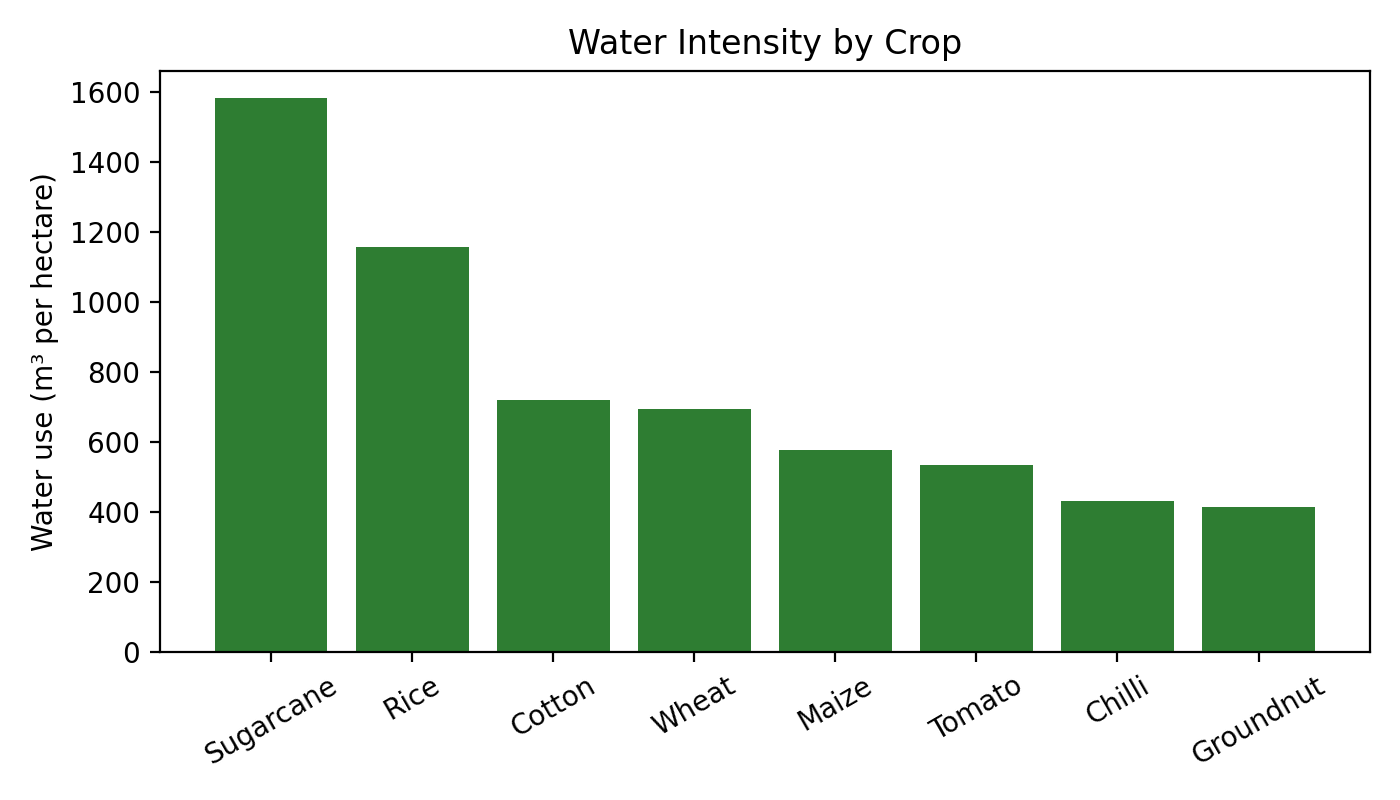
\includegraphics[width=0.78\textwidth]{figures/crop_intensity.png}
\caption{Water intensity by crop (m$^3$/ha), generated by the program.
  Sugarcane and rice stand clearly apart from the other six crops.}
\label{fig:crop}
\end{figure}

\subsection{Regional comparison and irrigation methods}
Warangal (850.4~m$^3$/ha), Karimnagar (828.2) and Nizamabad (790.6) are above the
overall average, while Medak (614.3) and Mahabubnagar (595.3) are well below it;
Warangal uses 43\% more water per hectare than Mahabubnagar. The three high-use
regions together consume 68.4\% of total water. Karimnagar has the largest absolute
consumption (302,320~m$^3$, 23.4\%) because it has the most irrigated area --- which
is exactly why intensity, not total, is the fair comparison. The differences are
mostly crop mix: rice and sugarcane make up 30.5\% of irrigated area in Warangal and
23.0\% in Karimnagar, but only 16.3\% in Nizamabad, which explains why Nizamabad ---
despite the highest regional water factor and the highest single sugarcane intensity
(1,829.1~m$^3$/ha) --- ranks third overall.

Flood irrigation uses 1,365.0~m$^3$/ha, compared with 707.0 for furrow, 487.7 for
sprinkler and 485.6 for drip (Table~\ref{tab:method}): flood is 2.8 times as
water-hungry as drip and supplies 41.6\% of all water. Because flood is used only for
the two most demanding crops, part of this gap is due to the crops themselves, not
only to the method.

\begin{table}[h]
\centering\small
\caption{Water consumption by region and by irrigation method.}
\label{tab:method}
\begin{tabular}{lrrrrr}
\toprule
Group & Records & Total (m$^3$) & Share (\%) & Area (ha) & m$^3$/ha \\
\midrule
\multicolumn{6}{l}{\textit{Region (ranked by intensity)}} \\
Warangal & 109 & 299,535.1 & 23.18 & 352.22 & 850.4 \\
Karimnagar & 113 & 302,320.0 & 23.39 & 365.02 & 828.2 \\
Nizamabad & 113 & 282,494.2 & 21.86 & 357.33 & 790.6 \\
Medak & 99 & 205,860.8 & 15.93 & 335.10 & 614.3 \\
Mahabubnagar & 116 & 202,130.9 & 15.64 & 339.56 & 595.3 \\
\midrule
\multicolumn{6}{l}{\textit{Irrigation method}} \\
Flood & 122 & 537,423.5 & 41.59 & 393.73 & 1,365.0 \\
Furrow & 138 & 305,508.3 & 23.64 & 432.14 & 707.0 \\
Sprinkler & 154 & 233,363.1 & 18.06 & 478.46 & 487.7 \\
Drip & 136 & 216,046.1 & 16.72 & 444.90 & 485.6 \\
\bottomrule
\end{tabular}
\end{table}

\subsection{High-consumption periods and crop-by-region patterns}
Water use is strongly seasonal (Figure~\ref{fig:month}). October is the peak month
(192,861~m$^3$, 14.9\%), followed by November (12.3\%) and June (11.8\%); together
these three months account for 39.0\% of annual use. By season, the kharif months
(June--October) use 54.0\%, rabi (November--March) 42.5\% and summer (April--May)
only 3.5\%; May is lowest at 0.8\%. The June and October--November peaks coincide
with rice and cotton sowing and the start of rabi crops, when many fields are
irrigated at once --- the point of greatest pressure on canal supply and groundwater.

\begin{figure}[h]
\centering
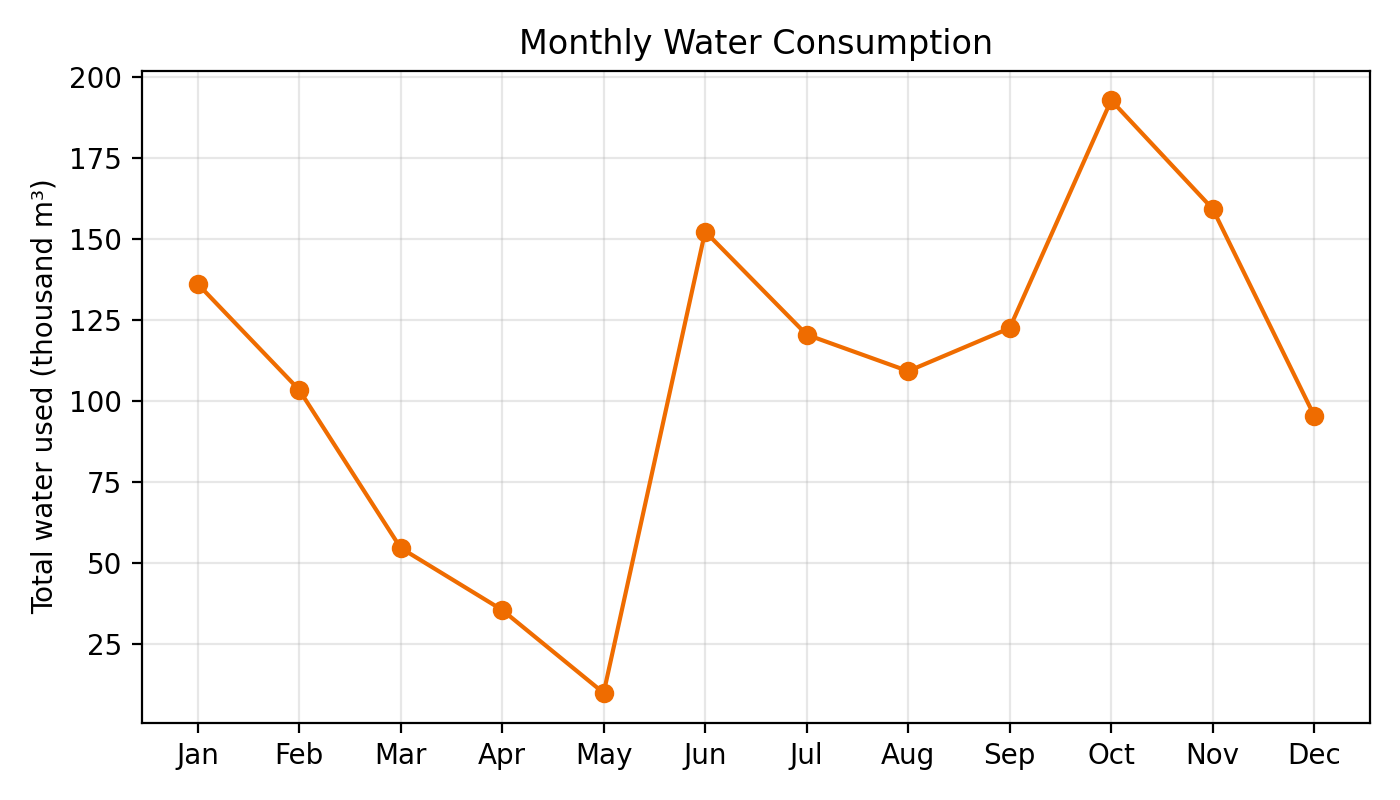
\includegraphics[width=0.78\textwidth]{figures/monthly_usage.png}
\caption{Monthly water consumption (thousand m$^3$), generated by the program.
  The June and October--November peaks dominate the year.}
\label{fig:month}
\end{figure}

The crop $\times$ region heatmap (Figure~\ref{fig:heat}) shows the same story at finer
grain. The hot spots are sugarcane in Nizamabad (1,829~m$^3$/ha), Warangal (1,748) and
Karimnagar (1,593), and rice in Karimnagar (1,475). The lowest cells are groundnut in
Medak (323), chilli in Mahabubnagar (357) and groundnut in Warangal (366). The same
crop can differ by 40--50\% between regions (rice ranges from 867 in Mahabubnagar to
1,475 in Karimnagar), which suggests that better practice in high-use regions could
bring them closer to the low-use ones. Four problem areas follow: (1)~10.1\% of raw
records were unusable, showing weak record-keeping; (2)~flood irrigation of rice and
sugarcane dominates water use; (3)~the June and October--November peaks overload
water sources; (4)~large same-crop differences between regions point to avoidable
over-irrigation.

\begin{figure}[h]
\centering
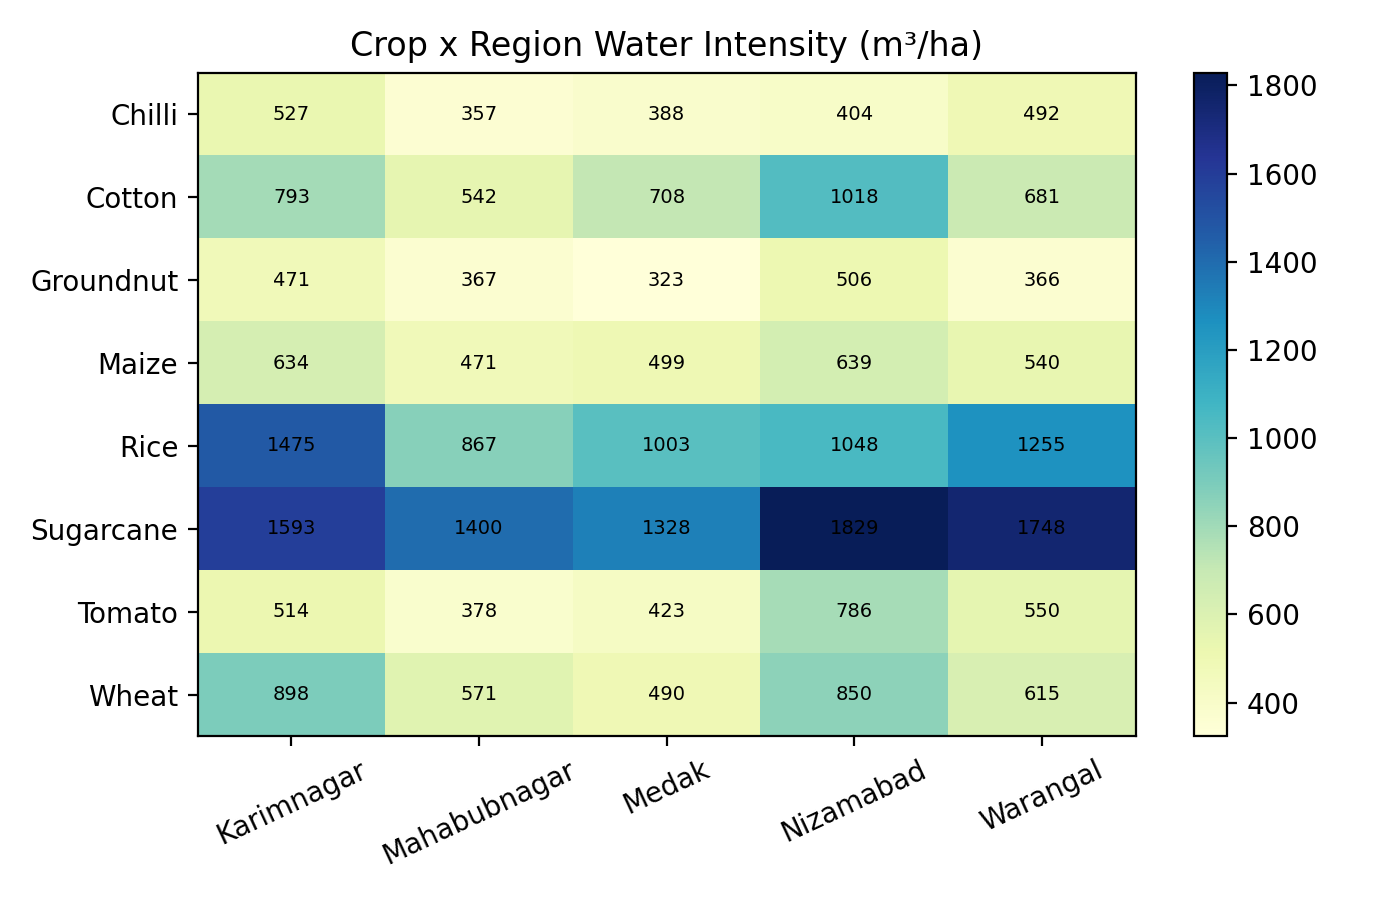
\includegraphics[width=0.78\textwidth]{figures/heatmap.png}
\caption{Crop $\times$ region water intensity (m$^3$/ha), generated by the program.
  Sugarcane is the darkest row in every region; groundnut and chilli are the lightest.}
\label{fig:heat}
\end{figure}

\section{Testing and Validation}
No tests existed in the original project, so a \texttt{tests/} suite using only the
standard library (\texttt{unittest}, no extra dependency) was added; it is run with
\texttt{python -m unittest discover -s tests -v}. Table~\ref{tab:tests} summarises it.
All 12 tests passed on the verified run. The end-to-end test runs the real program in
a fresh temporary directory and checks that all five charts, the cleaned CSV and the
headline totals (550 rows, 1,292,341.0~m$^3$) are produced.

\begin{table}[h]
\centering\small
\caption{Tests added and their outcome (12 tests, all passed).}
\label{tab:tests}
\begin{tabular}{ll}
\toprule
Area tested & Cases \\
\midrule
Cleaning & Normal row kept and typed; text normalisation; exact duplicate \\
         & Missing, negative, invalid-month and unknown-crop rows rejected \\
         & Non-numeric value rejected; $Q3+3\times IQR$ outlier rule \\
Stats & Intensity ranking and share arithmetic; monthly shares sum correctly \\
      & Crop $\times$ region cell value; drip rate returned by
        \texttt{potential\_saving} \\
End to end & Deterministic generation: seed 16 gives 612 rows, 550 clean \\
           & Fresh-directory run produces 5 charts, 4 summary CSVs, cleaned CSV \\
\bottomrule
\end{tabular}
\end{table}

Testing found one real bug, which was fixed rather than hidden: \texttt{clean\_data}
crashed with \texttt{IndexError} when \emph{every} input row was rejected, because it
indexed an empty intensities list to compute quartiles. A three-line guard now returns
an empty result with \texttt{clean\_rows = 0} in that case. The fix does not change any
result on the real data (the verified totals above are identical before and after it).
Two honest weaknesses remain and are documented, not fixed by rewriting the program:
\texttt{save\_csv} assumes at least one row, and duplicate detection compares raw rows
\emph{before} text normalisation, so two rows differing only by case or spacing are
not counted as duplicates. The statistics functions also expect cleaned, typed records;
passing raw CSV strings to them raises a type error, which is why the tests clean
first. The program was run with Python 3.12.3 and Matplotlib 3.6.3; the only dependency
is Matplotlib (\texttt{requirements.txt}).

\section{Recommendations and Action Plan}
Each recommendation below is linked to a measured problem area and uses proven
technology, implementable in stages:
\begin{enumerate}
  \item \textbf{Replace flood irrigation for rice and sugarcane:} alternate wetting and
        drying (AWD) for rice, drip (or furrow with mulching) for sugarcane. These two
        crops account for 41.6\% of water use, so this gives the largest saving.
  \item \textbf{Schedule around peak months:} stagger sowing and irrigation turns in
        June and October--November, irrigate at night or early morning to cut
        evaporation, and plan canal releases for these months.
  \item \textbf{Diversify crops in high-intensity regions:} in Warangal and Karimnagar,
        encourage maize, groundnut, chilli or pulses on part of the area now under
        rice and sugarcane.
  \item \textbf{Move vegetables to drip and cereals to sprinklers:} drip and sprinkler
        already use about 65\% less water per hectare than flood irrigation.
  \item \textbf{Irrigate by need, not by habit:} soil-moisture sensors or tensiometers,
        mulching and crop-stage schedules to stop over-irrigation.
  \item \textbf{Improve data quality:} flow meters, a standard digital record sheet,
        and validation with a script like this one before any analysis.
\end{enumerate}

\begin{table}[h]
\centering\small
\caption{Implementation action plan.}
\begin{tabular}{p{4.6cm}p{3.2cm}p{2.2cm}p{3.4cm}}
\toprule
Action & Responsible & Timeline & Measure of success \\
\midrule
Flow meters; standard record format; run analyzer monthly &
  Agriculture office, farmers & 0--3 months & Under 2\% invalid records \\
Train farmers in AWD and peak-month scheduling &
  Extension officers & 3--6 months & AWD fields adopted \\
Pilot drip / furrow with mulching for sugarcane in Warangal, Karimnagar &
  Farmers, irrigation dept., subsidy schemes & 6--12 months &
  m$^3$/ha reduced vs.\ baseline \\
Coordinate canal releases and turn-based irrigation for June, Oct--Nov &
  Water user associations & Before next kharif & Peak-month use flattened \\
Review with the analyzer; expand to all regions &
  Agriculture office & 12 months & Targeted saving achieved \\
\bottomrule
\end{tabular}
\end{table}

The headline saving is a planning estimate, not a promise: a 30\% reduction in flood
water (537,423.5~m$^3$) equals 161,227~m$^3$, or 12.5\% of total use. Actual savings
must be confirmed by field measurement, because crop and method effects are entangled
(Section~3).

\section{Challenges, Limitations and Lessons Learned}
Challenges encountered were: no real farm-level dataset was available, so a simulated
dataset had to be constructed honestly and labelled as such; crop and method are
strongly linked, limiting causal claims; rainfall, soil, groundwater and yield data
were absent; the outlier rule is a statistical choice that could remove a few genuine
high values; and only one year was analysed. Lessons learned: cleaning takes real
effort (one in ten rows unusable, each rule counted and reported); normalising by area
is essential, since totals alone mislead; looking beyond rankings explains causes
(Warangal's rank came from crop mix, not only regional conditions); dictionaries and
\texttt{defaultdict} made grouping short and readable, and separate functions kept
the program testable; and charts made seasonal peaks and hot spots far clearer than
tables alone.

\section{Conclusion and Future Scope}
A short Python program can turn raw irrigation records into practical guidance. After
cleaning 612 records down to 550 valid ones, the analysis found that sugarcane and
rice are the main water-intensive crops, Warangal and Karimnagar the highest-intensity
regions, and October, November and June the high-consumption periods, with flood
irrigation the least efficient method. Switching flood-irrigated fields to AWD or drip,
spreading demand across peak months, diversifying crops and installing flow meters
could cut water use by around 12.5\% under a conservative assumption, and the same
program can be applied to real records to support water-conservation decisions.

Realistic future work, in order of value: replace simulated data with real farm, canal
or smart-meter records; add rainfall, soil, groundwater depth and crop yield to compute
water productivity (kg per m$^3$); use multi-year data for trend analysis and
forecasting with pandas, NumPy or machine learning; build a web dashboard so extension
officers can upload data and view charts; connect IoT soil-moisture sensors for
real-time irrigation alerts; and add cost and energy analysis to estimate the payback
of drip systems.

\section{Mapping of Program Outcomes and SDGs}
\subsection{Program Outcomes}
\begin{table}[h]
\centering\small
\caption{PO mapping (condensed; full wording is in the companion Word report).}
\begin{tabular}{>{\raggedright\arraybackslash}p{3.6cm}
  >{\raggedright\arraybackslash}p{11.3cm}}
\toprule
PO & Relevance to this case study \\
\midrule
PO1 Engineering Knowledge & Programming fundamentals and basic statistics applied
  to an agricultural problem. \\
PO2 Problem Analysis & Water-intensive crops, high-use regions and peak months
  identified from records and their causes interpreted. \\
PO3 Design of Solutions & Reusable analyzer designed; AWD, drip, scheduling and
  diversification proposed. \\
PO4 Investigations & Records collected, validated, compared across four dimensions
  and conclusions drawn from evidence. \\
PO5 Tool Usage & Python 3, \texttt{csv} and \texttt{collections}, Matplotlib. \\
PO6 Engineer and World & Addresses water scarcity and sustainable farming for
  farmers, communities and the environment. \\
PO7 Ethics & Farm codes anonymise farms; the simulated dataset is stated openly
  and never presented as real measurements. \\
PO8 Team Work & Three members shared data preparation, coding, analysis and writing. \\
PO9 Communication & Findings documented in tables, charts and plain recommendations. \\
PO10 Project Management & Phased action plan with timelines, responsibilities and
  cost considerations for drip and meters. \\
PO11 Life-Long Learning & Encourages further learning in data analysis,
  visualisation and precision agriculture. \\
\bottomrule
\end{tabular}
\end{table}

\subsection{Sustainable Development Goals}
Only the four most relevant SDGs are claimed: \textbf{SDG 2 (Zero Hunger)} ---
efficient irrigation supports sustainable agriculture and farm incomes;
\textbf{SDG 6 (Clean Water and Sanitation)} --- directly targets water-use efficiency
and reduced pressure on groundwater and canal supplies; \textbf{SDG 12 (Responsible
Consumption and Production)} --- identifies wasteful irrigation and promotes efficient
use of a scarce resource; \textbf{SDG 13 (Climate Action)} --- helps farms adapt to
erratic rainfall and reduces pumping energy and emissions.

\section*{References}
\addcontentsline{toc}{section}{References}
\begin{thebibliography}{9}
\bibitem{fao56} R.~G. Allen, L.~S. Pereira, D.~Raes and M.~Smith,
  \emph{Crop Evapotranspiration: Guidelines for Computing Crop Water Requirements},
  FAO Irrigation and Drainage Paper 56, FAO, Rome, 1998.
\bibitem{aquastat} Food and Agriculture Organization of the United Nations,
  AQUASTAT --- FAO's Global Information System on Water and Agriculture,
  \url{https://www.fao.org/aquastat}.
\bibitem{python} Python Software Foundation, Python 3 Documentation:
  \texttt{csv} --- CSV File Reading and Writing; \texttt{collections} --- Container
  datatypes, \url{https://docs.python.org/3/}.
\bibitem{mpl} J.~D. Hunter, ``Matplotlib: A 2D graphics environment,''
  \emph{Computing in Science \& Engineering}, vol.~9, no.~3, pp.~90--95, 2007.
\bibitem{mckinney} W.~McKinney, \emph{Python for Data Analysis}, 3rd~ed.,
  O'Reilly Media, 2022.
\bibitem{irri} International Rice Research Institute, Alternate Wetting and Drying,
  Rice Knowledge Bank, \url{http://www.knowledgebank.irri.org}.
\bibitem{un} United Nations, \emph{Transforming our World: The 2030 Agenda for
  Sustainable Development} (Goals 2, 6, 12 and 13), \url{https://sdgs.un.org}.
\end{thebibliography}
\noindent\textit{Note: the dataset used in this study was simulated by the
accompanying Python program (seed 16).}

\appendix
\section{Demonstration: Program Output}
Figure~\ref{fig:term} shows the verified run: the program was executed from a clean
directory with Python 3.12.3, generated 612 records, cleaned them to 550, printed the
tables summarised in Sections~6--7, and saved five charts and four summary CSVs in
\texttt{output/}. The image is a rendered transcript of that actual run log, cropped
to the cleaning report and headline totals; the full log and tables are in the
repository. The complete program (343 lines, including the empty-input guard described
in Section~7) is in the repository as \texttt{water\_usage\_analyzer.py} and is not
reprinted here, to keep this report within its page limit. The program, its tests
and this report are published at
\url{https://github.com/Taraka-Ramarao-D/Agricultural-Water-Usage-Analyzer}
(see the project README).

\begin{figure}[h]
\centering
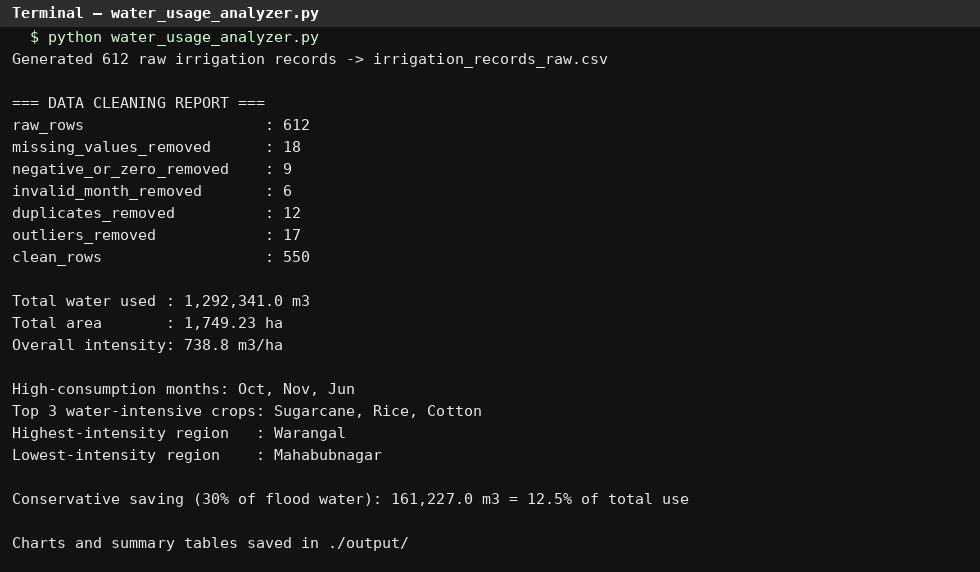
\includegraphics[width=0.95\textwidth]{figures/terminal_output.png}
\caption{Terminal output of the verified run (cleaning report and headline totals).}
\label{fig:term}
\end{figure}

\end{document}
